% TikZ Architecture Pipeline Diagram for "The DOM Serialization Gap"
% Depicts the 5-stage transformation pipeline, pruning bottlenecks, and auxiliary channels.

\begin{figure*}[t]
\centering
\resizebox{\linewidth}{!}{%
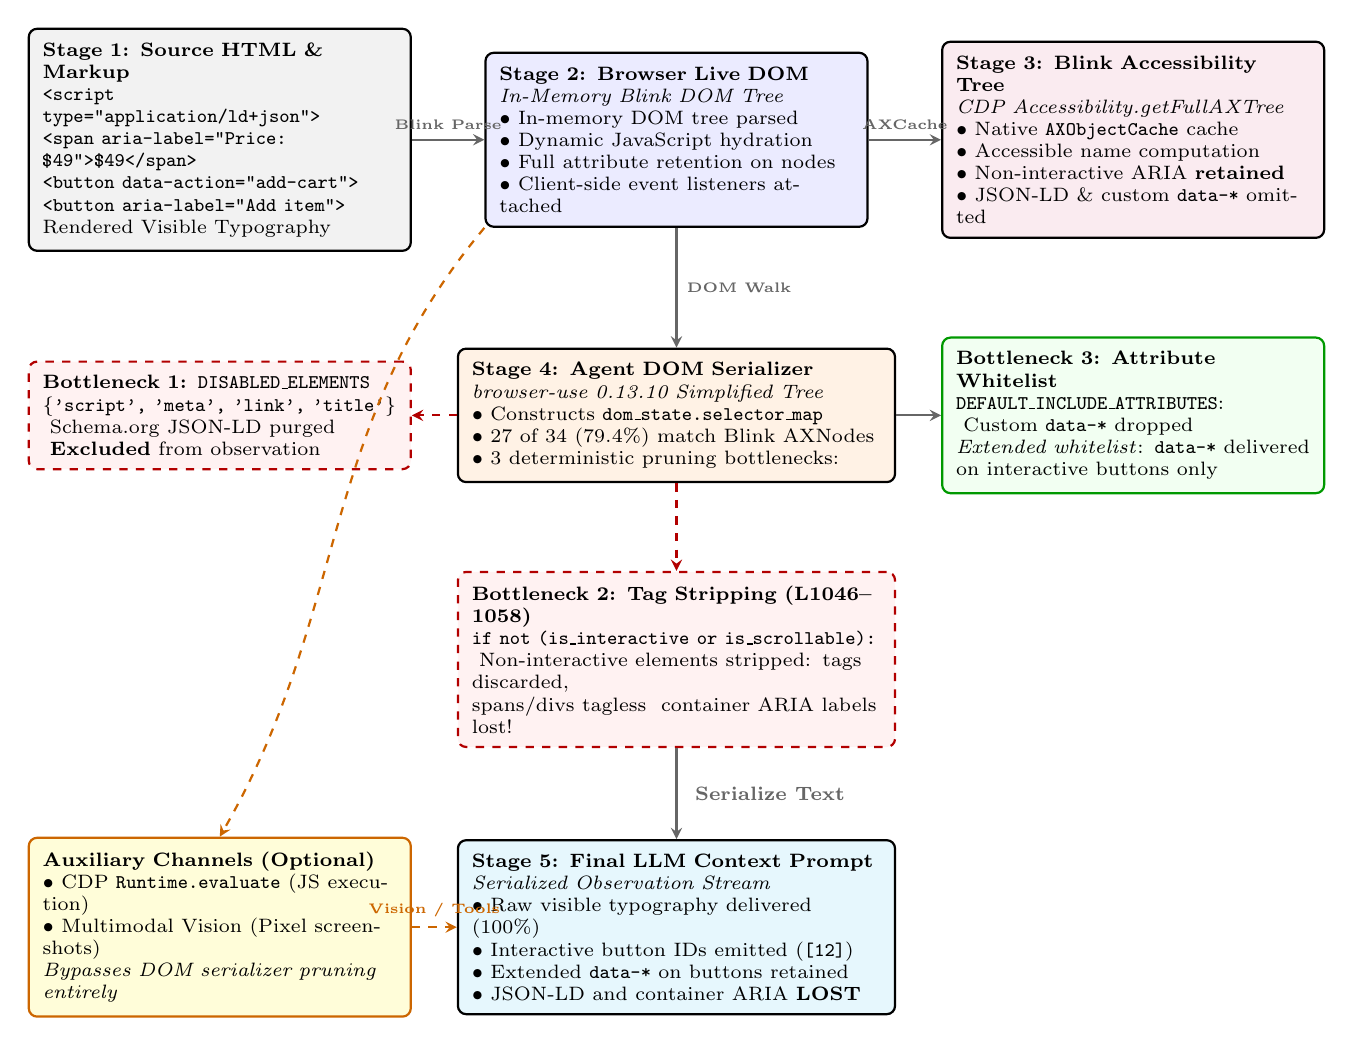
\begin{tikzpicture}[
    box/.style={draw, rounded corners=3pt, thick, align=left, fill=blue!5, font=\scriptsize, inner sep=5pt},
    prunebox/.style={draw=red!70!black, dashed, rounded corners=3pt, thick, align=left, fill=red!5, font=\scriptsize, inner sep=5pt},
    survivebox/.style={draw=green!60!black, rounded corners=3pt, thick, align=left, fill=green!5, font=\scriptsize, inner sep=5pt},
    arrow/.style={->, >=stealth, thick, color=gray!80!black},
    prunearrow/.style={->, >=stealth, dashed, thick, color=red!70!black}
]

% ── Tier 1: Browser Runtime & Representations (Stages 1, 2, 3) ────────────────
\node[box, fill=gray!10, text width=4.5cm] (s1) at (0, 0) {
\textbf{Stage 1: Source HTML \& Markup}\\
\texttt{<script type="application/ld+json">}\\
\texttt{<span aria-label="Price: \$49">\$49</span>}\\
\texttt{<button data-action="add-cart">}\\
\texttt{<button aria-label="Add item">}\\
Rendered Visible Typography
};

\node[box, fill=blue!8, text width=4.5cm] (s2) at (5.8, 0) {
\textbf{Stage 2: Browser Live DOM}\\
\textit{In-Memory Blink DOM Tree}\\
$\bullet$ In-memory DOM tree parsed\\
$\bullet$ Dynamic JavaScript hydration\\
$\bullet$ Full attribute retention on nodes\\
$\bullet$ Client-side event listeners attached
};

\node[box, fill=purple!8, text width=4.5cm] (s3) at (11.6, 0) {
\textbf{Stage 3: Blink Accessibility Tree}\\
\textit{CDP Accessibility.getFullAXTree}\\
$\bullet$ Native \texttt{AXObjectCache} cache\\
$\bullet$ Accessible name computation\\
$\bullet$ Non-interactive ARIA \textbf{retained}\\
$\bullet$ JSON-LD \& custom \texttt{data-*} omitted
};

% ── Tier 2: Agent Serializer & Pruning Bottlenecks (Stage 4) ──────────────────
\node[prunebox, text width=4.5cm] (b1) at (0, -3.5) {
\textbf{Bottleneck 1: \texttt{DISABLED\_ELEMENTS}}\\
\texttt{\{'script', 'meta', 'link', 'title'\}}\\
$\implies$ Schema.org JSON-LD purged\\
$\implies$ \textbf{Excluded} from observation
};

\node[box, fill=orange!10, text width=5.2cm] (s4) at (5.8, -3.5) {
\textbf{Stage 4: Agent DOM Serializer}\\
\textit{browser-use 0.13.10 Simplified Tree}\\
$\bullet$ Constructs \texttt{dom\_state.selector\_map}\\
$\bullet$ 27 of 34 ($79.4\%$) match Blink AXNodes\\
$\bullet$ 3 deterministic pruning bottlenecks:
};

\node[survivebox, text width=4.5cm] (b3) at (11.6, -3.5) {
\textbf{Bottleneck 3: Attribute Whitelist}\\
\texttt{DEFAULT\_INCLUDE\_ATTRIBUTES}:\\
$\implies$ Custom \texttt{data-*} dropped\\
\textit{Extended whitelist}: \texttt{data-*} delivered\\
on interactive buttons only
};

% ── Tier 3: Bottleneck 2 (Tag Stripping) ──────────────────────────────────────
\node[prunebox, text width=5.2cm] (b2) at (5.8, -6.6) {
\textbf{Bottleneck 2: Tag Stripping (L1046--1058)}\\
\texttt{if not (is\_interactive or is\_scrollable):}\\
$\implies$ Non-interactive elements stripped: tags discarded,\\
spans/divs tagless $\implies$ container ARIA labels lost!
};

% ── Tier 4: Model Observation Context & Auxiliary Channels (Stage 5) ─────────
\node[box, fill=yellow!15, draw=orange!80!black, text width=4.5cm] (aux) at (0, -10.0) {
\textbf{Auxiliary Channels (Optional)}\\
$\bullet$ CDP \texttt{Runtime.evaluate} (JS execution)\\
$\bullet$ Multimodal Vision (Pixel screenshots)\\
\textit{Bypasses DOM serializer pruning entirely}
};

\node[box, fill=cyan!10, text width=5.2cm] (s5) at (5.8, -10.0) {
\textbf{Stage 5: Final LLM Context Prompt}\\
\textit{Serialized Observation Stream}\\
$\bullet$ Raw visible typography delivered ($100\%$)\\
$\bullet$ Interactive button IDs emitted (\texttt{[12]})\\
$\bullet$ Extended \texttt{data-*} on buttons retained\\
$\bullet$ JSON-LD and container ARIA \textbf{LOST}
};

% ── Connective Arrows ─────────────────────────────────────────────────────────
\draw[arrow] (s1) -- node[above, font=\tiny\bfseries] {Blink Parse} (s2);
\draw[arrow] (s2) -- node[above, font=\tiny\bfseries] {AXCache} (s3);
\draw[arrow] (s2) -- node[right, font=\tiny\bfseries] {DOM Walk} (s4);

\draw[prunearrow] (s4) -- (b1);
\draw[arrow] (s4) -- (b3);
\draw[prunearrow] (s4) -- (b2);
\draw[arrow] (b2.south) -- node[right=3pt, font=\scriptsize\bfseries] {Serialize Text} (s5.north);

\draw[arrow, dashed, color=orange!80!black] (s2.south west) to[out=230, in=60] (aux.north);
\draw[arrow, dashed, color=orange!80!black] (aux.east) -- node[above, font=\tiny\bfseries] {Vision / Tools} (s5.west);

\end{tikzpicture}%
}
\caption{End-to-end architecture of the autonomous browser agent observation pipeline (\texttt{browser-use 0.13.10}). Web markup transitions across five discrete representations from source HTML to final LLM prompt. Three deterministic pruning bottlenecks in Stage 4 selectively purge structured Schema.org JSON-LD, strip non-interactive WAI-ARIA annotations, and filter custom developer attributes. Auxiliary channels (CDP JavaScript evaluation or visual screenshots) bypass serializer pruning entirely.}
\label{fig:pipeline_architecture}
\end{figure*}
